\section{Supplementary results}
\label{sec:sup-res.}

\subsection{Summary variable statistics}
\label{sec:sum-var-stat}
Figures~\ref{fig:tauuo_stats_america}~&~\ref{fig:tauvo_stats_america} which
are analogous to Figure~\ref{fig:ssh_stats_america}, but for $\tau_u$ and
$\tau_v$.

\begin{figure*}[htb!]
    \centering
    \includegraphics[width=0.6\linewidth]{../surge/plots/stats_points_plottauuo.pdf}
       \hspace{0pt} \includegraphics[width=0.285\linewidth]{../surge/plots/stats_points_plottauuo_1.pdf}
    \vspace{-7pt}
    \caption{\texttt{tauuo}, $\tau_u$ for \texttt{tyr}, \texttt{eUS}}
   \label{fig:tauuo_stats_america}

   \includegraphics[width=0.6\linewidth]{../surge/plots/stats_points_plottauvo.pdf}
      \hspace{0pt} \includegraphics[width=0.285\linewidth]{../surge/plots/stats_points_plottauvo_1.pdf}
   \vspace{-7pt}
   \caption{\texttt{tauvo}, $\tau_v$ for \texttt{tyr}, \texttt{eUS}}
  \label{fig:tauvo_stats_america}
\end{figure*}


\begin{figure*}[htb!]
    \centering
    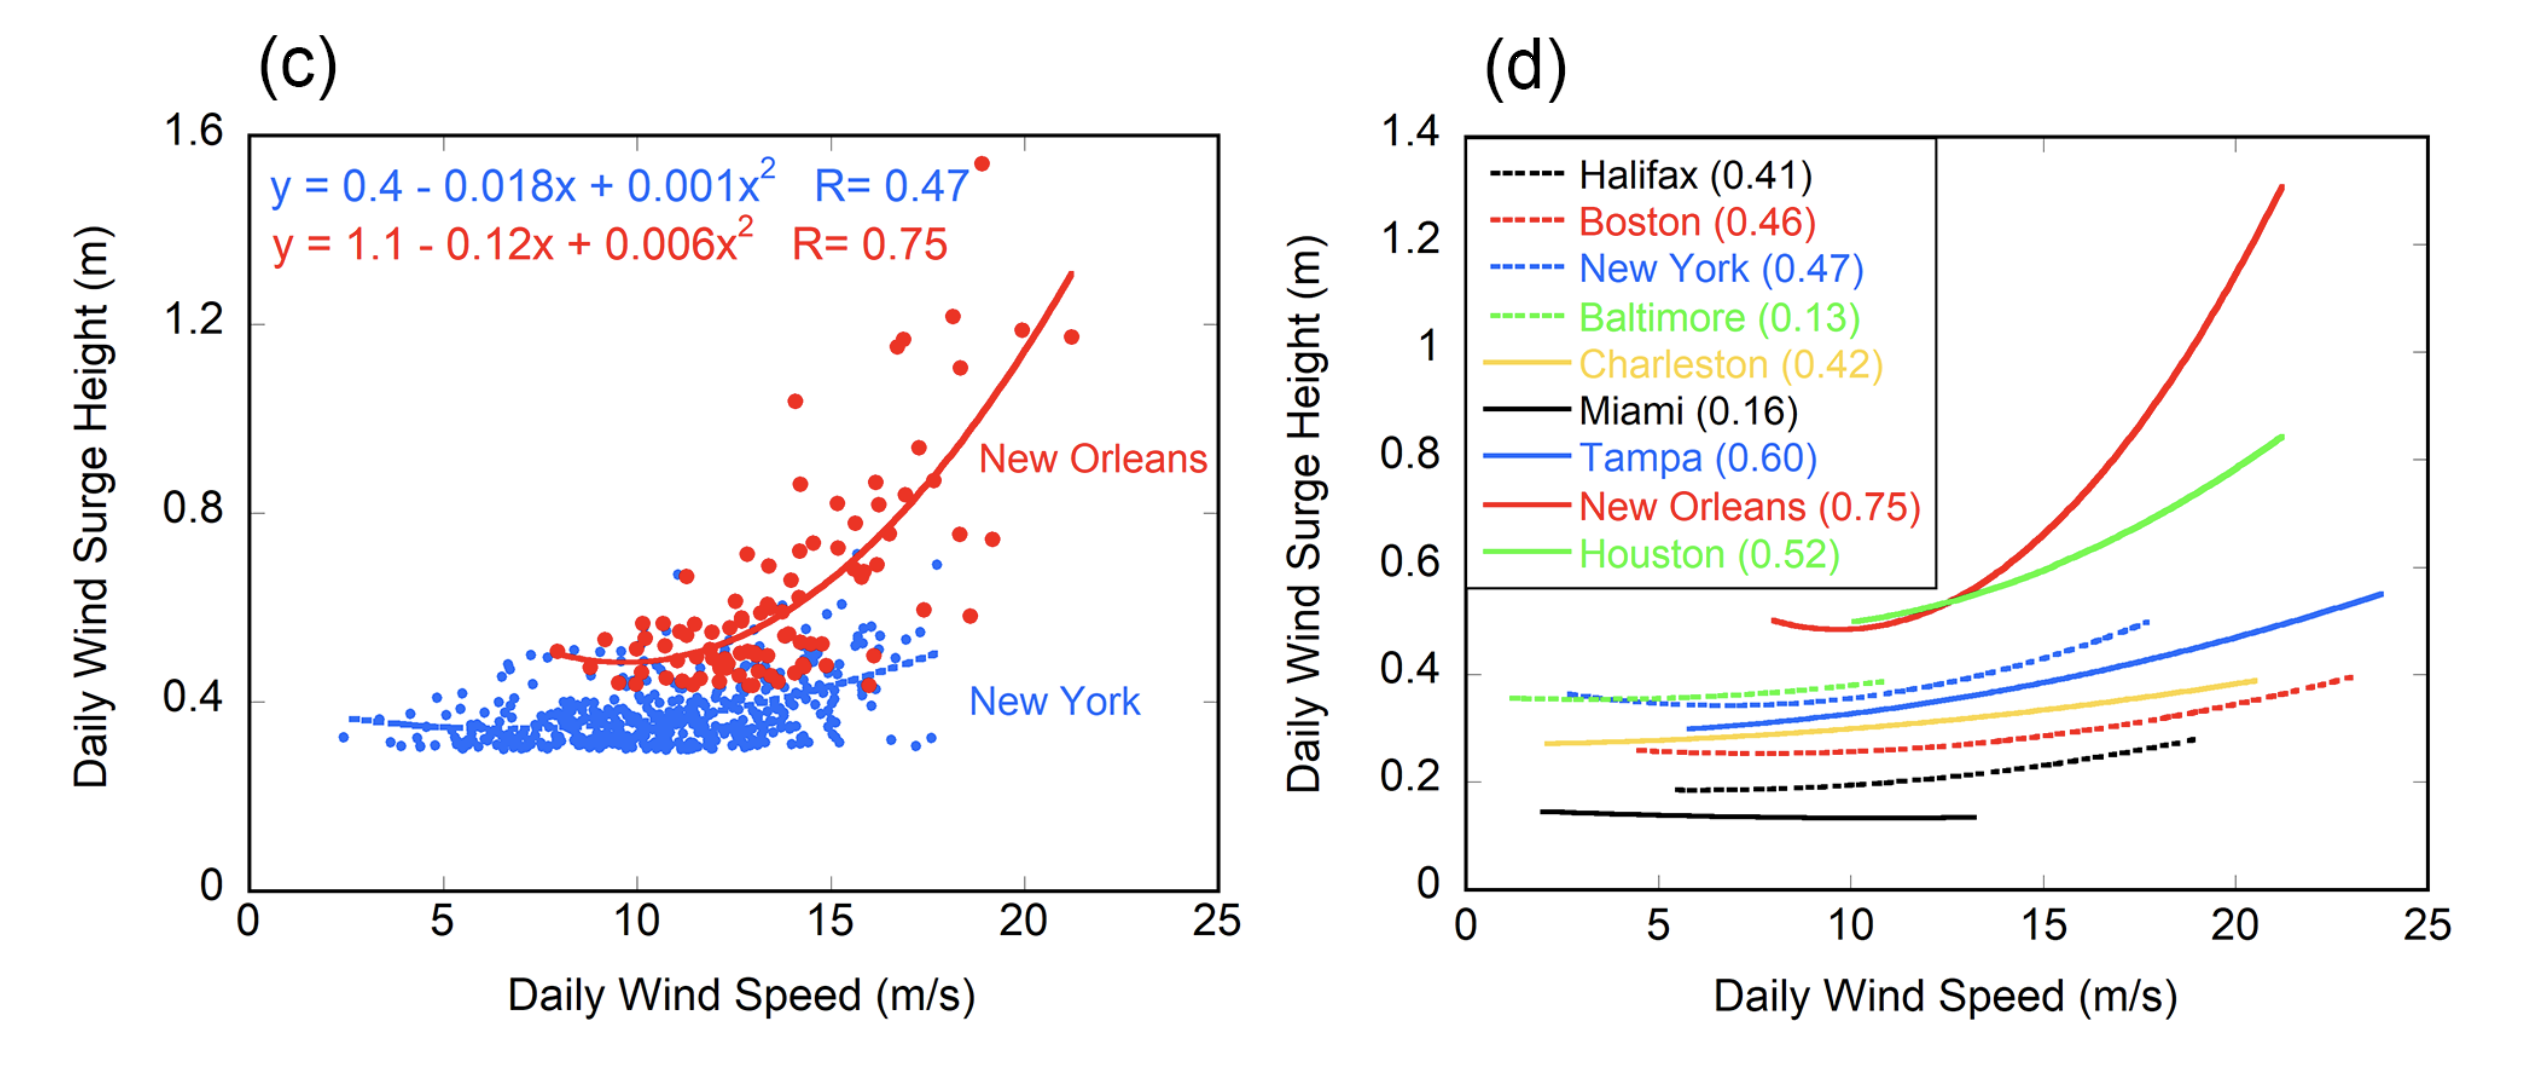
\includegraphics[width=0.8\linewidth]{images/example-images/yin-responsiveness.png}
    \vspace{-7pt}
    \caption{Figure 10c \& 10d in Yin et al.~2020~\cite{ZannaPreprint}. }
   \label{fig:yin-responsiveness}

   \includegraphics[width=0.8\linewidth]{../surge/plots/score-plot/score_plot.pdf}
   \vspace{-7pt}
   \caption{Linear Regression of $ \Delta \eta$ against $|U|^2$ for $ \Delta\eta>0$.
   Only generalises for the most vulnerable points. Most variance not modelled.}
  \label{fig:simple-responsiveness-results}
\end{figure*}


\paragraph{Gaussian processes (GPs)}
\begin{itemize}
\item Equations 2.13-2.14 in GPML~\cite{williams2006gaussian}.
\begin{align}
m(\mathbf{x})&=&\mathbb{E}[f(\mathbf{x})] % \tag{Mean}
\\
k\left(\mathbf{x}, \mathbf{x}^{\prime}\right)&=&\mathbb{E}
\left[(f(\mathbf{x})-m(\mathbf{x}))\left(f\left(\mathbf{x}^{\prime}\right)
-m\left(\mathbf{x}^{\prime}\right)\right)\right]
%\tag{Covariance}
\\
f(\mathbf{x})& \sim& \mathcal{G} \mathcal{P}\left(m(\mathbf{x}),
 k\left(\mathbf{x}, \mathbf{x}^{\prime}\right)\right)%\tag{GP}
\end{align}
\item Can assume $m(\mathbf{x})=0$ without terrible consequences.
 \item Thought should be put into the form of $k\left(\mathbf{x},
  \mathbf{x}^{\prime}\right)$~\cite{duvenaud2014automatic}.
\item GPs assume that there is a Gaussian error around each point,
      but this is often not the case in real variables.
      However, it is often possible to transform to
      a space where this is the case, Krige there,
      and then transform
      back~\cite{snelson2004warped}.\footnote{\url{http://mlg.eng.cam.ac.uk/zoubin/papers/gpwarp.pdf}}
      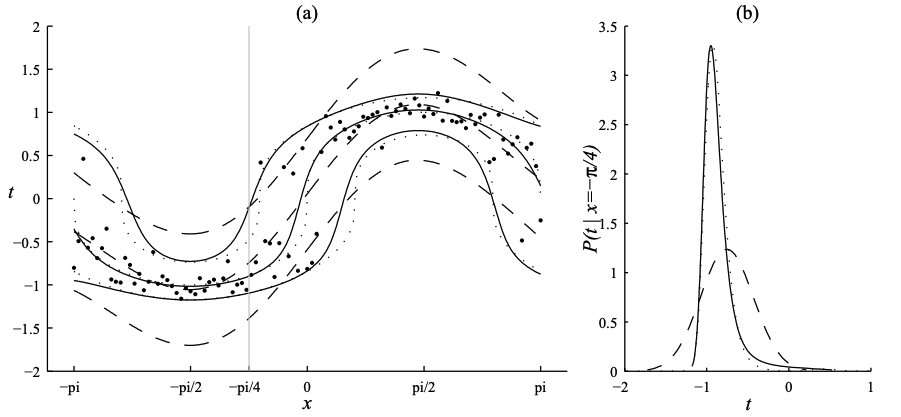
\includegraphics[width=\linewidth]{images/example-images/warped-example.png}\\
      \textit{Figure 1 from~\cite{snelson2004warped}}
\item Lewis Fry Richardson (1948) showed that the estimates
      of deaths during a war had
      symmetric error bars in logarithmic space~\cite{richardson1948variation}.
      \cite{snelson2004warped}~mentions this as a common trick.
 \end{itemize}

\begin{figure*}[htb!]
    \centering
    \includegraphics[width=0.85\linewidth]{../surge/plots/stats_points_plot_2.pdf}
    \vspace{-7pt}
    \caption{An attempt to check whether there are discontinuities
     over the special points, to explain the offsets of the means.
     The points are ordered from Eastport (EP) (furthest north east),
     to Rockport (RP) (furthest south west). From the plot it is visible
     that there is a low frequency annual component to each signal, and that
     the excursions are more common during autumn and winter, with
     relative calm in spring.}
    \label{fig:individual_zos}
    \includegraphics[width=0.85\linewidth]{../surge/plots/ahh/ahhhhh4.pdf}
    \vspace{-7pt}
    \caption{Mean SSH over points of the US coast over the two year period. There is a strong yearly periodicity in $\eta$ (and its variance?).
     Kriged with a Sobol quasirandom subsample~\cite{sobol1967distribution} of 6000 time points.
     }
    \label{fig:gauss-mean}
\end{figure*}

\begin{figure}[htb!]
\includegraphics[width=\linewidth]{../surge/plots/vc_bath_list.pdf}
\vspace{-25pt}

\caption{Isobaths plotted for \texttt{vc}.}
\label{fig:bath}
\includegraphics[width=\linewidth]{../surge/plots/vc_distance_isobath.pdf}
\vspace{-25pt}

\caption{Distance to isobaths from points on \texttt{vc}.}
\label{fig:vc_isobath}
\includegraphics[width=\linewidth]{../surge/plots/vc_isobath_correlate.pdf}
\vspace{-25pt}

\caption{The correlation matrix between the different isobath's distance's to
\texttt{vc}.}
\label{fig:vc_isobath}
\end{figure}


\begin{figure}[htb!]
\centering
\includegraphics[width=\linewidth]{../surge/plots/vc_angle_heatmap.pdf}
\caption{Normal bearing, $B^{\prime}$, along \texttt{vc}.

         }
\label{fig:angle_heatmap}

\includegraphics[width=\linewidth]{../surge/plots/vc_derivative_heatmap.pdf}
\caption{Convexity metric along \texttt{vc}.
         The three panels above show bay like concavity in blue, and convexity
         in red. At the largest $\sigma$ only the largest headlands visible (C), whereas the smallest bays are visible at a lower
        $\sigma$ (A).
}
\label{fig:derivative}
\end{figure}


\subsubsection{1D model with TC PI theory}
\label{sec:1d-hurr}
To explore the impact that an increased amount of greenhouse gasses might have
on the system, consider a single layer model of the atmosphere, described by the
set of four simultaneous equations.

\begin{eqnarray}
F_{\mathrm{solar}} =& F_{\mathrm{atm}} + F_{\mathrm{ground}}\tau_{\mathrm{IR}}\\
F_{\mathrm{solar}}(1-\tau_{\mathrm{vis}}) =& 2F_{\mathrm{atm}} + F_{\mathrm{ground}}(\tau_{\mathrm{IR}}-1)\\
F_{\mathrm{ground}} = & F_{\mathrm{solar}}(\tau_{\mathrm{vis}}) +F_{\mathrm{atm}}  \\
F_{\mathrm{ground}} = & \sigma T_{\mathrm{ground}}{}^4 \\
F_{\mathrm{atm}} = & \sigma T_a{}^{4},
\end{eqnarray}

where F is the fluxes from the different areas of the model,
$ \tau_{\mathrm{IR}}$ and $\tau_{\mathrm{vis}}$ are the opacity of the atmosphere
to infrared and visible radiation respectively.
This leads to the solution

\begin{equation}
T_{\mathrm{ground}} = \left( \frac{F_{\mathrm{solar}}}{\sigma}\frac{(1+\tau_{\mathrm{vis}})}{(1+\tau_{\mathrm{IR}})}\right)^{1/4},
\end{equation}

which shows that when $\tau_{\mathrm{IR}}$, i.e.~the ammount of greenhouse gasses,
is increased, this leads to an increase in the temperature of the (sea) surface (c. $T_s$).
When using the Stefan-Boltzmann relation,

\begin{equation}
F_{\mathrm{atm}} = \sigma T_a{}^{4},
\end{equation}

we can further find that the

\begin{equation}
T_{\mathrm{atm}}^{4}=T_{\mathrm{ground}}^4\frac{(1-\tau_{\mathrm{vis}}\tau_{\mathrm{IR}})}{(1+\tau_{vis})}
\end{equation}

so that the temperature of the atmosphere (approximately equivalent to $T_{o}$)
decreases as the amount of greenhouse gases are increased.


One can then use \ref{eq:PI} and see that as the nominator has increased, and the
denominator has decreased, the potential intensity is expected to increase with the
amount of greenhouse gases, $\tau_{\mathrm{IR}}$, in the atmosphere.

